
\section{Grafos}
Un grafo consiste en dos conjuntos finitos: un conjunto no vac\'io de
 v\'ertices y un conjunto de aristas, donde cada arista esta asociada 
 a uno o dos v\'ertices llamados puntos extremos\cite{SUSANNAS.EPP2012}. 
 Se dice que una arista incide sobre cada uno de sus puntos extremos, 
 dos aristas que inciden en el mismo punto se llaman adyacentes y el 
 v\'ertice en el que no incide ninguna arista se llama 
 aislado\cite{SUSANNAS.EPP2012}, En la figura \ref{fig:igrafo} se
 presenta un grafo que muestra las acciones dosponibles con el 
 teclado y rat\'on.
 
\begin{figure}[h]
\centering
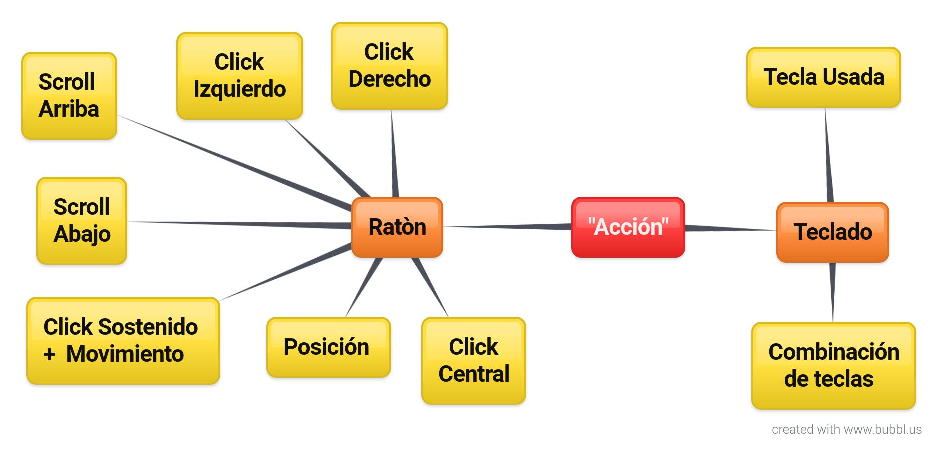
\includegraphics[width=0.8\columnwidth]{chap3/Imagenes/Grafo.eps}
\caption{Ejemplo de un grafo.}
\label{fig:igrafo}
\end{figure}


\subsection{Grafo Dirigido}
Un grafo dirigido se define por ser un grafo donde cada arista es un 
 par ordenado asignando la direcci\'on del primer elemento mencionado 
 al segundo\cite{SUSANNAS.EPP2012}. \'este tipo de grafo se puede 
 representar, en t\'erminos de programaci\'on,  como una lista enlazada, 
 la cual es ``una colecci\'on lineal de objetos de una clase autoreferenciada, 
 conocidos como nodos'' \cite{deitel2008java}, a \'estas solo se les puede 
 referenciar por el primer nodo, sin embargo, como cada elemento tiene la 
 referencia al siguiente se puede acceder a todos los elementos de la lista, 
 la ventaja ofrecida es la posibilidad de crear una lista de dimensi\'on 
 variable, por lo que es usada cuando se desconoce la cantidad total de 
 elementos a introducir\cite{deitel2008java}, otro ejemplo ser\'ia un 
 aut\'omata finito determinista como el presentado en la imagen
 \ref{fig:igrafoD}, en el cual se puede apreciar la diferencia con el grafo 
 por mostrar la direcci\'on de las aristas con una flecha, en lugar de usar 
 solo una recta.
 
\begin{figure}[h]
\centering
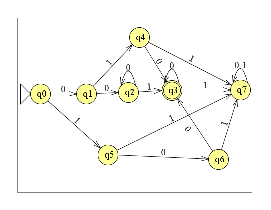
\includegraphics[width=0.8\columnwidth]{chap3/Imagenes/GrafoDirigido.eps}
\caption{Ejemplo de un grafo dirigido.}
\label{fig:igrafoD}
\end{figure}


\subsection{Teor\'ia de \'arboles}
En t\'erminos matem\'aticos un \'arbol es un grafo $T$ el cual se puede definir de
 la siguiente forma\cite{SUSANNAS.EPP2012}:

\begin{itemize}
	\item ``Un grafo se llama \'arbol si y solo si, est\'a libre de circuitos y
	 es conexo.''
	\item ``Un v\'ertice de grado 1 en $T$ se denomina un v\'ertice terminal (o
	 una hoja).''
	\item ``Un v\'ertice de grado superior a 1 en $T$ es un v\'ertice interno (o
	 un v\'ertice de rama).''
\end{itemize}


Los \'arboles son muy usados en la actualidad ya que permiten  darle sentido a
 la informaci\'on contenida, gracias a la asociatividad, parentizaci\'on y
 prioridad que este permite de manera impl\'icita. Entre sus usos m\'ultiples en
 el \'area de la inform\'atica se pueden destacar los  siguientes; relaciones
 entre m\'odulos de programaci\'on, \'arboles de decisi\'on en inteligencia artificial
 y representaciones gram\'aticas\cite{gutierrez1999estructuras}.  

Una forma de ver a un \'arbol puede ser como un solo nodo, est\'e recibe el nombre
 de  nodo ra\'iz, al cual se le puede enraizar un sinf\'in de \'arboles lo que da
 origen  a un \'arbol con otras caracter\'isticas, dependiendo del resultado se le
 puede clasificar en alguno de los modelos existentes, por ejemplo; \'arbol 
 general o \'arbol binario\cite{gutierrez1999estructuras},el mostrado en la figura
 \ref{fig:iarbol}, es un \'arbol binario que representa la jerarqu\'ia e 
 interconexi\'on entre varios procesadores. 

\begin{figure}[h]
\centering
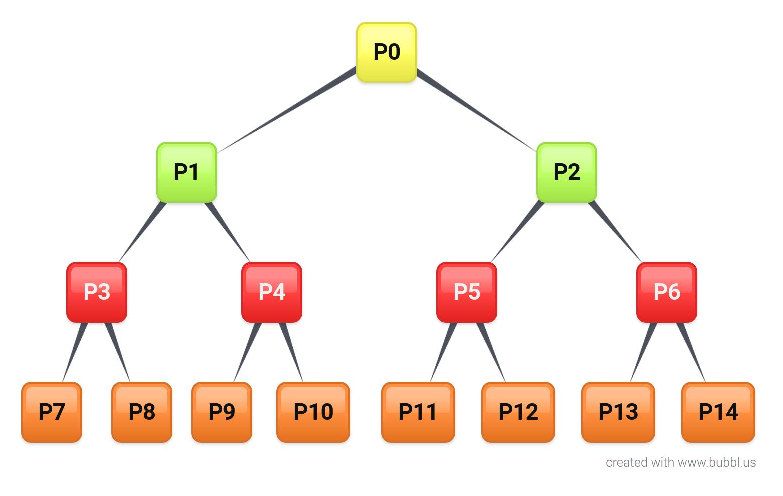
\includegraphics[width=0.8\columnwidth]{chap3/Imagenes/Arbol.eps}
\caption{Ejemplo de un \'arbol.}
\label{fig:iarbol}
\end{figure}

El \'arbol general es un modelo con una cantidad indeterminada de nodos hijos,
 mientras que el \'arbol binario es un caso particular del \'arbol general ya que
 este tiene la caracter\'istica de tener siempre en cada nodo 2 nodos hijos como
 m\'aximo, cabe mencionar que este es uno de los modelos a mas usados, as\'i como
 el ultimo caso mencionado, hay\'arboles que tienen una cantidad fija de nodos
 hijos, de manera general estos son llamados arboles n-arios
 \cite{gutierrez1999estructuras}.